\documentclass{article}
\usepackage{fontspec}
\usepackage{polyglossia}
\setdefaultlanguage{french}
\usepackage[a4paper,margin=1cm]{geometry}

\usepackage{amsmath}
\usepackage{amssymb}
\usepackage{array}
\usepackage{auto-pst-pdf}
\usepackage{booktabs}
\usepackage{cite}
\usepackage{graphicx}
\usepackage{lmodern}
\usepackage{marvosym}
\usepackage{mathrsfs}
\usepackage{minted}
\usepackage{multicol}
\usepackage{multirow}
\usepackage{paralist}
\usepackage{schemabloc}
\usepackage{siunitx}
\usepackage{soul}
\usepackage{tikz}
\usepackage[european,cuteinductors,siunitx]{circuitikz}
\usepackage{url,hyperref}
\usepackage{verbatim}
\usepackage{xunicode,xltxtra}

\title{
\includegraphics{../../images/inp-enseeiht} \\ ~ \\ ~ \\ ~ \\ ~ \\ BE CAN-CNA}
\author{François Pierron \& Guilhem Saurel}
\date{\oldstylenums{\today}}

\begin{document}

\begin{titlepage}
    \setcounter{page}{0}
    \maketitle
    \thispagestyle{empty}
\end{titlepage}

\paragraph{Déterminer le nombre de composants (résistances, capacités et interrupteurs) nécessaires pour \textbf{M=2} et \textbf{K=4} (avec N-bits=M-bits+K-bits).}

~

Si $M=2$, on a besoin de $2^M=4$ résistances, et si $K=4$ il nous faut $K+1=5$ condensateurs.

Pour les interrupteurs, il nous en faut

\begin{itemize}
    \item $4+1$ pour les résistances
    \item $K\times 2$ pour les condensateurs
    \item $1$ pour $S_F$
\end{itemize}

Ce qui fait environ 13 interrupteurs.

\paragraph{Réaliser un interrupteur CMOS fonctionnant sur toute la gamme du signal à convertir de 0v à $V_{ref}$. On prendra $V_{ref} = V_{dd} = 5$V.}

~

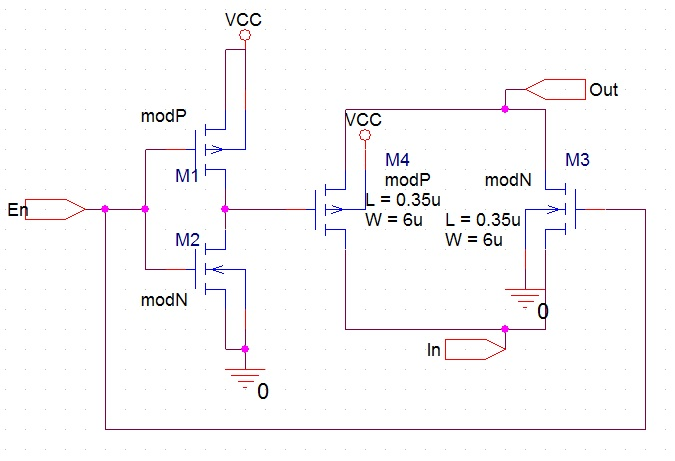
\includegraphics[width=\linewidth]{becancna/interrupteur.jpg}

\newpage

\paragraph{Tracer $R_{on} = f(V_e)$ avec un $V_{gs}$ maximum ($R_{on}$: résistance à l’état passant).}

~

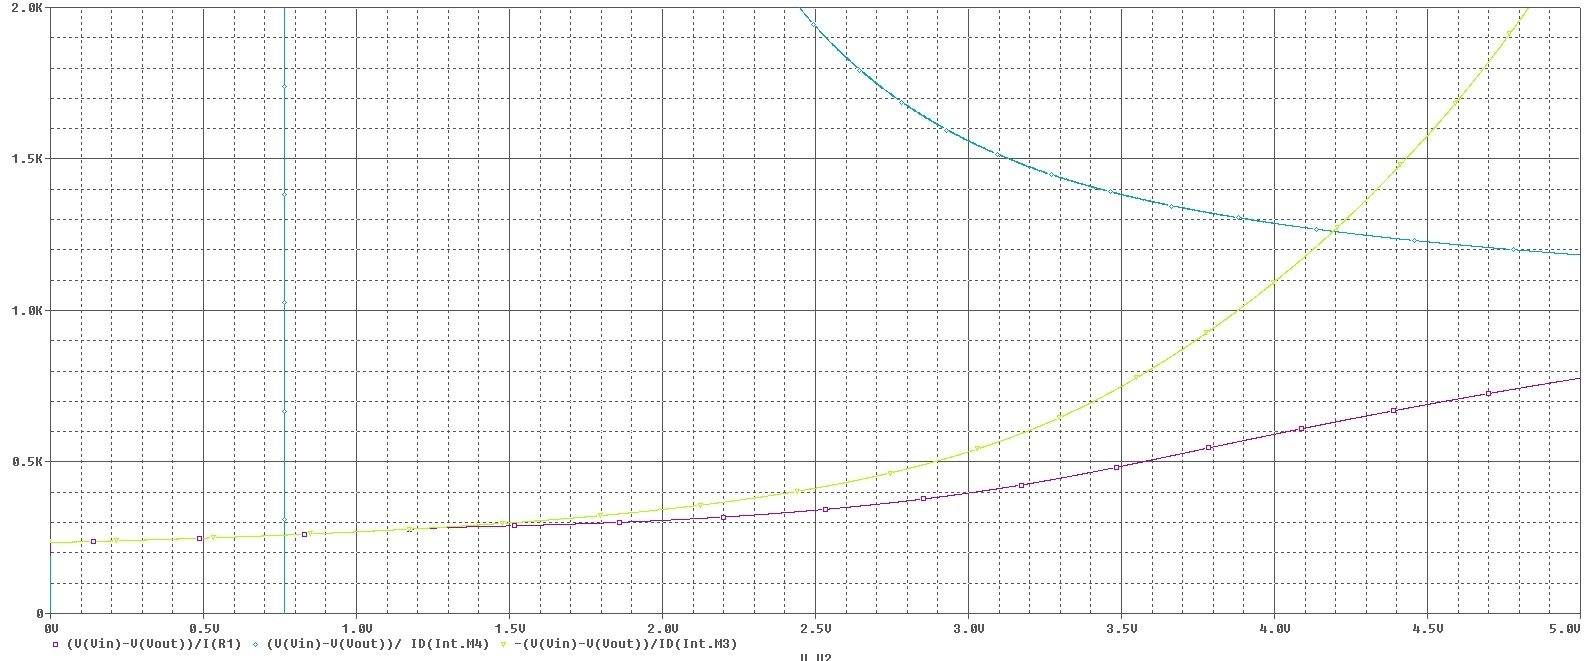
\includegraphics[width=\linewidth]{becancna/Ron.jpg}

\paragraph{Réaliser un multiplexeur 2 voies (utilisant l’interrupteur précédent).}

~

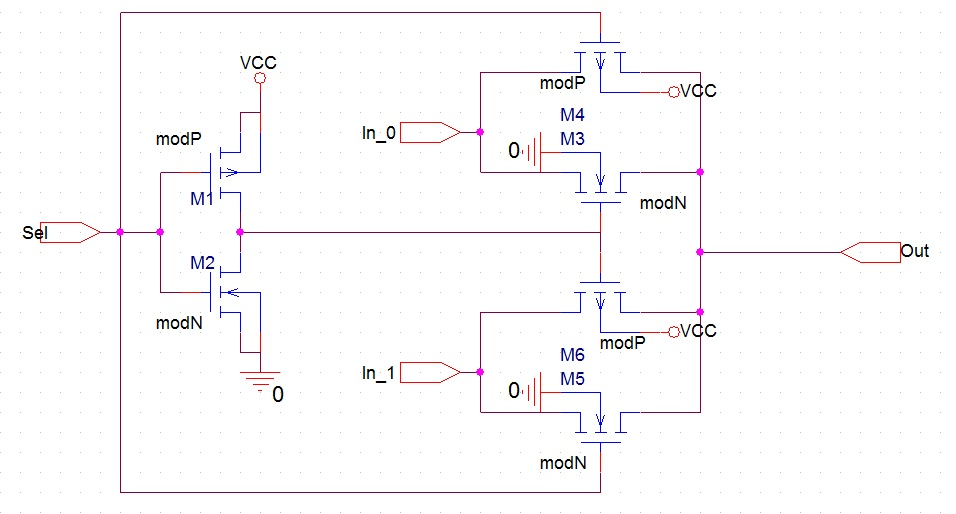
\includegraphics[width=\linewidth]{becancna/MUX.jpg}

\paragraph{Réaliser un convertisseur 6-bits utilisant un amplificateur idéal}

~

Le contrôle des cinq interupteurs qui sélectionnent le bon pont diviseur est assez simple à concevoir:

\begin{itemize}
    \item $\phi b_0 b_1$
    \item $\phi b_0$
    \item $\phi b_0 \oplus b_1$
    \item $\phi \bar b_0$
    \item $\phi \bar b_0 \bar b_1$
\end{itemize}

\newpage

Naturellement, on peut factoriser $\phi$.

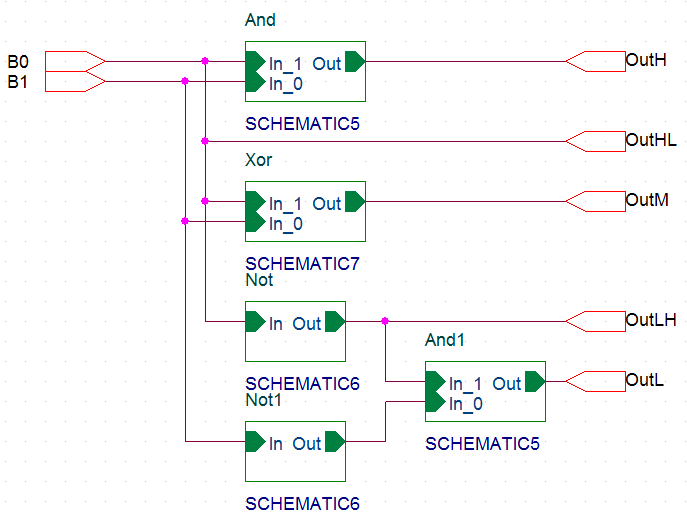
\includegraphics[width=\linewidth]{becancna/dec2.png}

Avant de passer à la suite, on peut tester son fonctionnement:

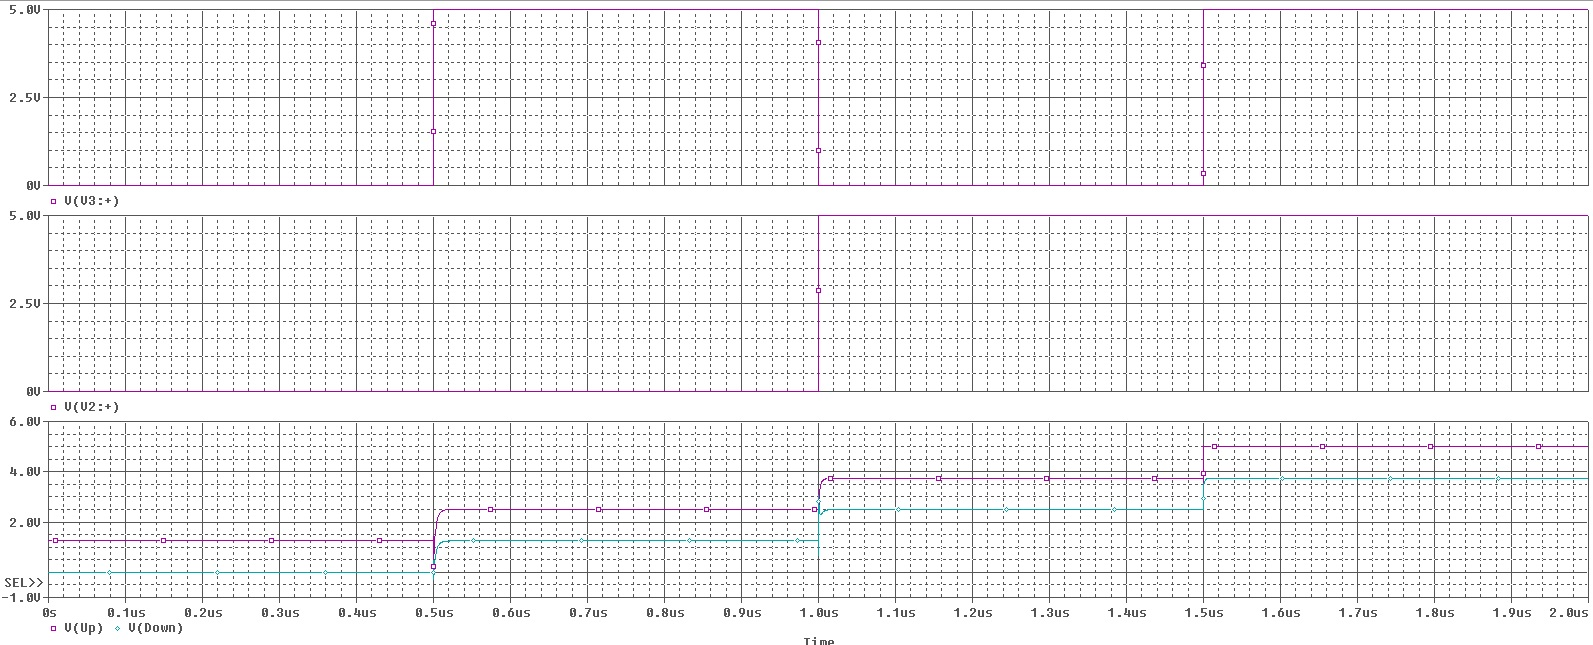
\includegraphics[width=\linewidth]{becancna/decodeur.jpg}

Pour le reste:

$S_A = \bar S_B = b_1$

$S_{M+i} = b_{M+1}$

$S_F = \phi$

\newpage

On a alors notre circuit (sans l’amplificateur, qui ne servait visiblement qu’à nous gêner…):

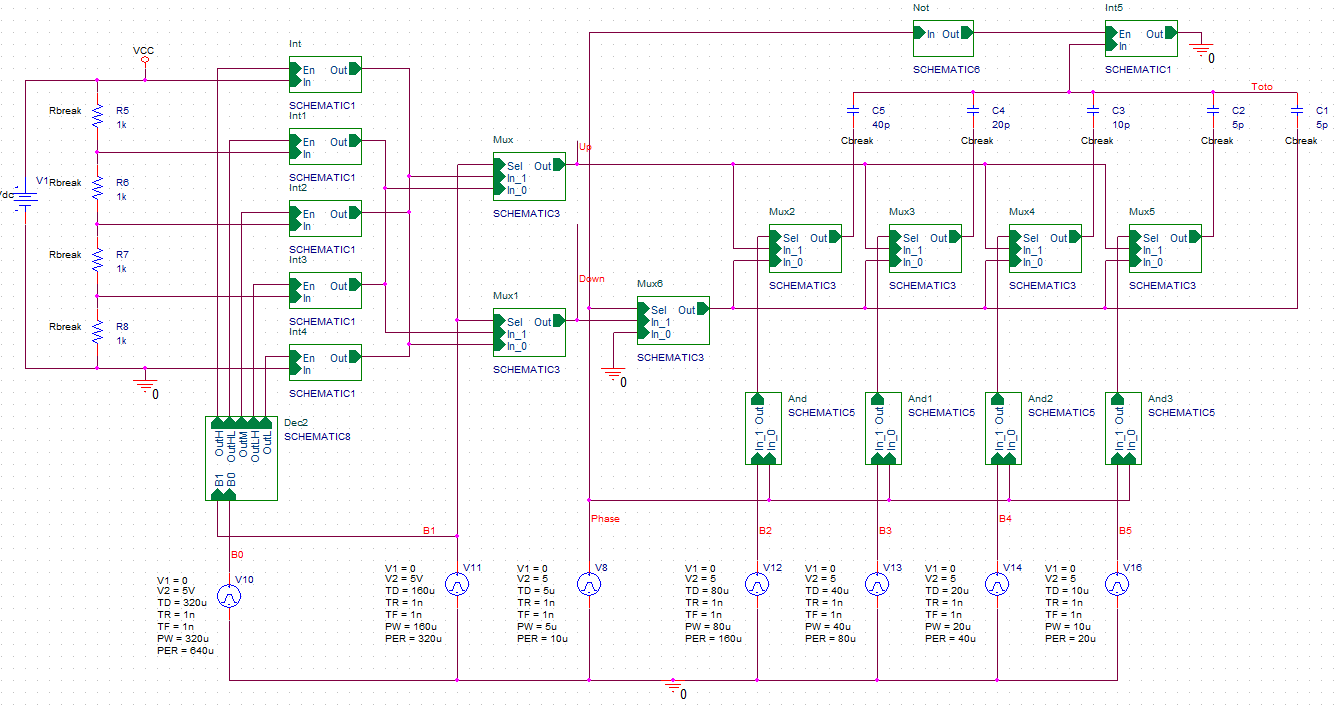
\includegraphics[width=\linewidth]{becancna/circuit.png}

Et sa simulation:

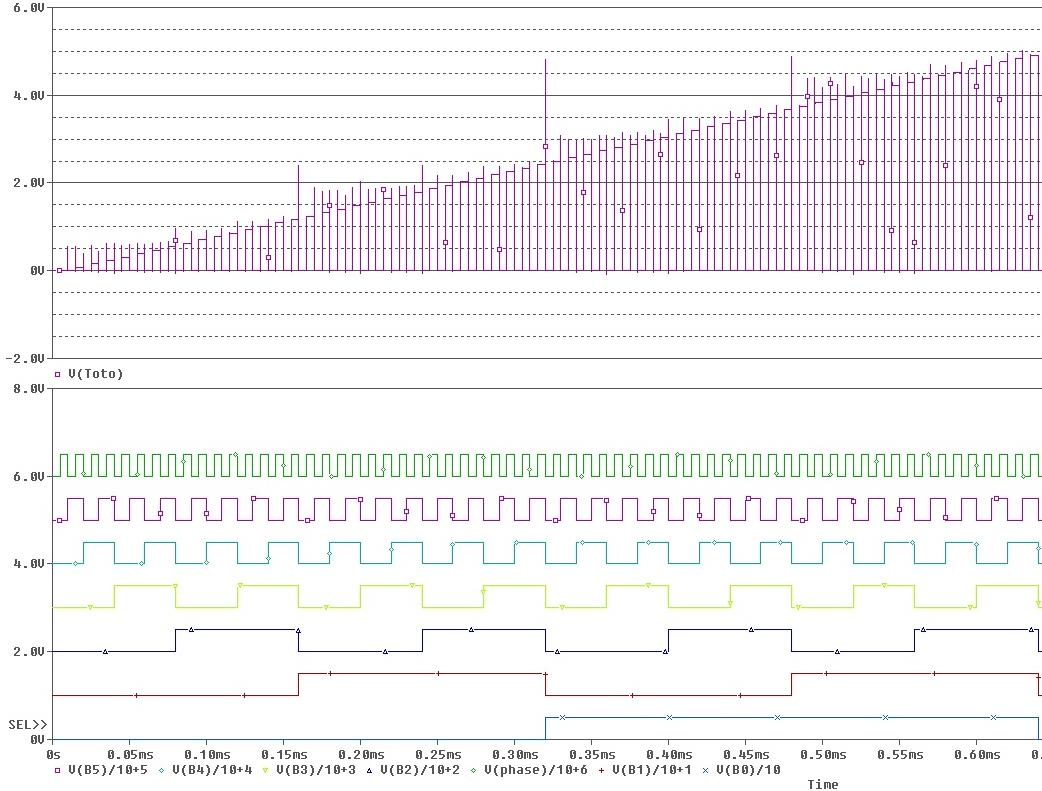
\includegraphics[width=\linewidth]{becancna/convertisseur.jpg}

\newpage

\paragraph{À l’aide de simulations de Monte-Carlo, déterminer les variations relatives max $\cfrac{\Delta R}{R} = \cfrac{\Delta C}{C}$ pour obtenir une INL et DNL inférieures à ½ LSB}

~

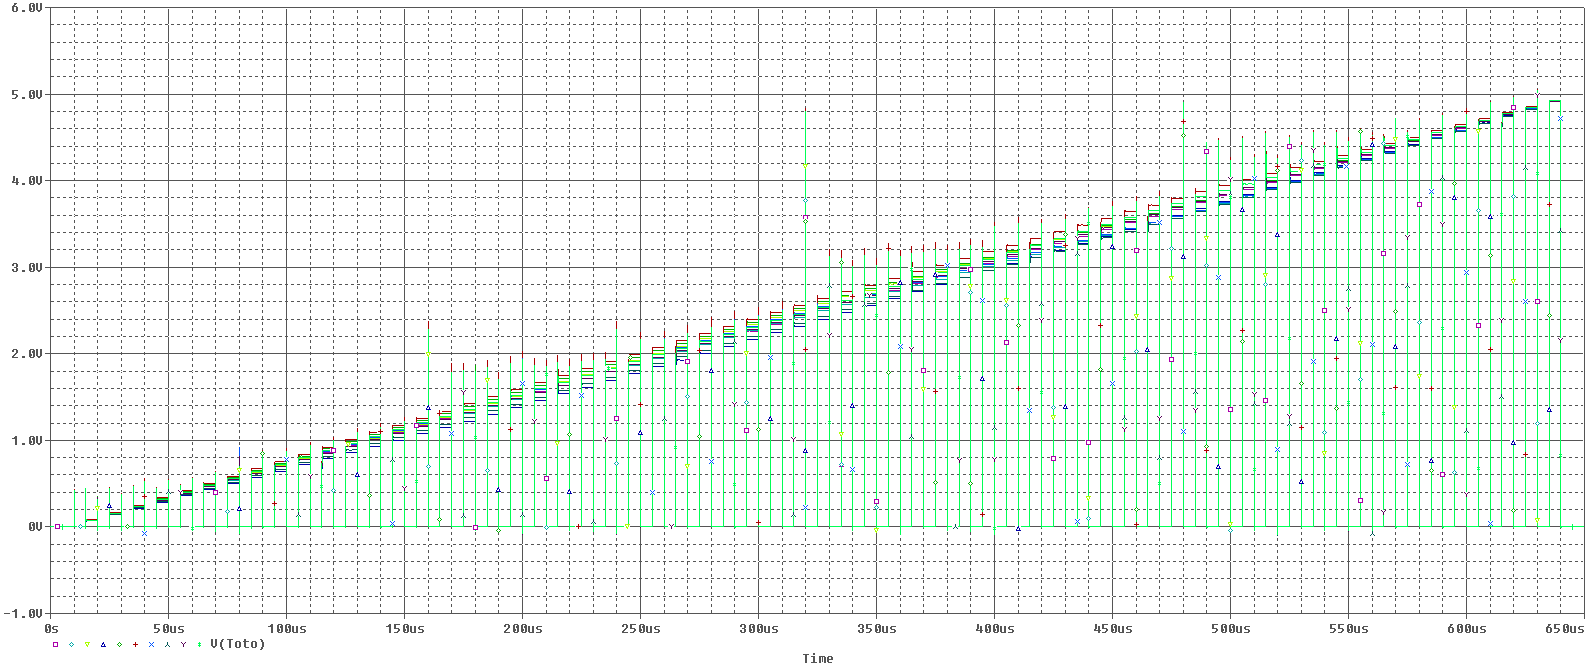
\includegraphics[width=\linewidth]{becancna/monte_carlo.png}


En refaisant des simulations pour des tolérances de 10\%, 5\% et 1\%, on se rend compte que la différence absolue maximale entre la simulation minimale et la simulation maximale est inférieure à ½LSB seulement pour 1\%.

\end{document}

